\documentclass[12pt,twoside]{report}
\pagenumbering{roman}

\usepackage{graphicx}
\usepackage{subcaption}
\usepackage[utf8]{inputenc}
\usepackage[german]{babel}
% for units
\usepackage{siunitx}

\usepackage{hyperref}
\hypersetup{
  colorlinks=true,
  linkcolor=blue,
  filecolor=magenta,      
  urlcolor=cyan,
}

\urlstyle{same}


\begin{document}
% CONSTANTS BEGIN
\newcommand{\githubrepo}{\href{https://github.com/Pierrefha/ees-buggy-project}{GitHub-Repository}}
\newcommand{\referenzcode}{\href{https://github.com/tomfclarke/adafruit-motor-hat-cpp-library}{Referenz-Code}}
% \newcommand{\github_repo}{\href{https://github.com/Pierrefha/ees-buggy-project}{GitHub-Repository}}
% \newcommand{\referenz_code}{\href{https://github.com/tomfclarke/adafruit-motor-hat-cpp-library}{Referenz-Code}}
\begin{titlepage}
    \begin{center}
        \vspace*{1cm}
            
        \Huge
        \textbf{Lernportfolio}

        \vspace{1.5cm}
            
        \normalsize
        \textbf{Pierre Dahmani pd1528s 3215892\\
        Jens Peter Dennigmann jd8389s 3190025 \\
        Leonhard Kipp lk2149s 3188047\\}
            
        \vfill
            
        EES Buggy-Projekt 
        \vspace{0.8cm}
            
        %% TODO Add title pic
        %% \includegraphics[width=0.4\textwidth]{university}
        \pagebreak
    \end{center}
\end{titlepage}

% TODO Inhaltsverzeichnis

\begin{section}{Aufbau des Buggy}

\begin{figure}[h!]
  \centering
  \captionsetup[subfigure]{labelformat=empty}
  \begin{subfigure}{0.45\linewidth}
    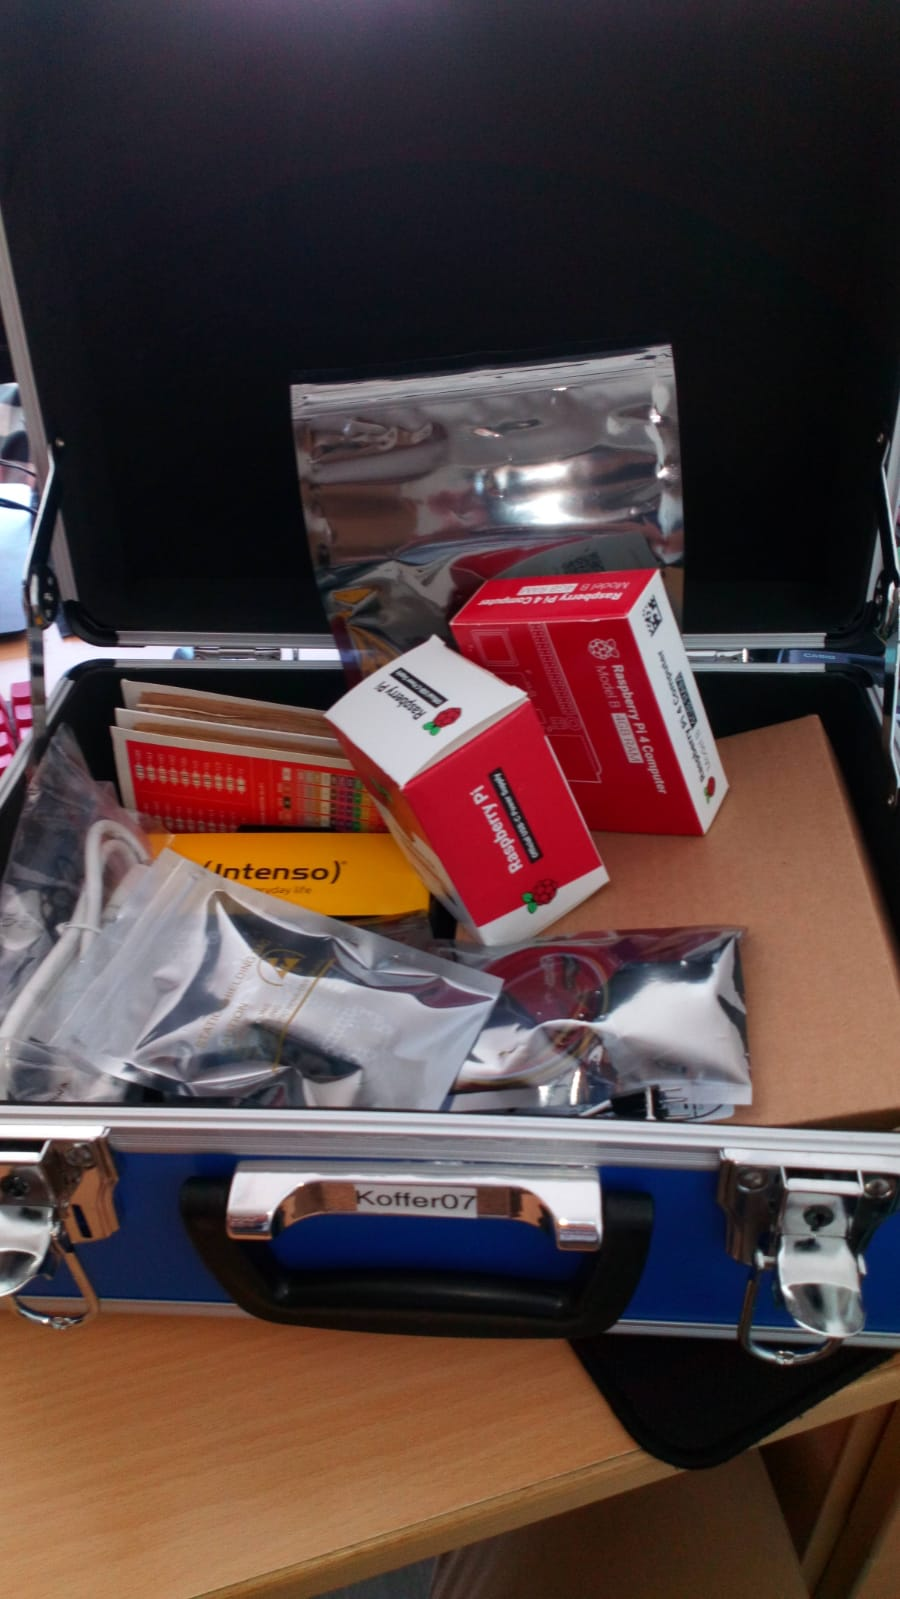
\includegraphics[width=\linewidth]{lernportfolio_assets/Buggy_Koffer.jpeg}
    \caption{Der Buggy vor dem Aufbau.}
  \end{subfigure}
  \begin{subfigure}{0.45\linewidth}
    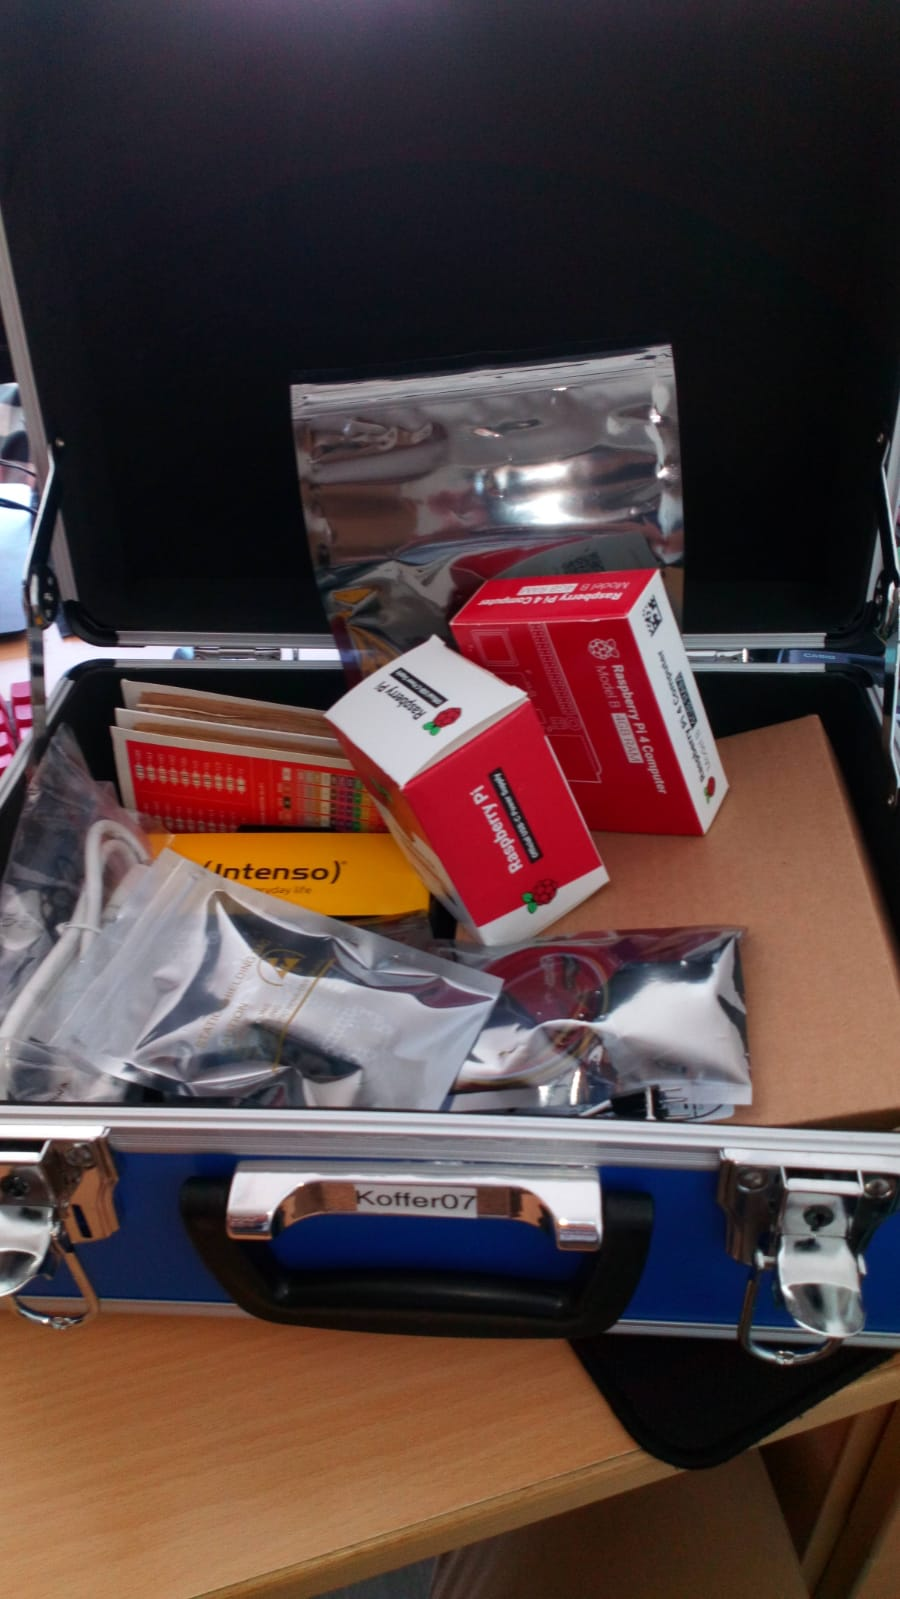
\includegraphics[width=\linewidth]{lernportfolio_assets/Buggy_Koffer.jpeg}
    \caption{Und danach.}
  \end{subfigure}
\end{figure}

Der Buggy wurde vor der Herausgabe des Arbeitsauftrages zusammengebaut. Zwischenschritte sind daher nicht bildlich festgehalten. 

Der Zusammenbau des Buggies verlief problemlos. Der Text ist insgesamt verständlich geschrieben und war eine große Unterstützung.

% Wollen wir das aufnehmen?
% Im Text ist der Genetiv von ``der Buggy'' durchgehend ``des Buggies''. Mit Verweis
% auf \url{https://www.duden.de/rechtschreibung/Buggy} ist der korrekte - und
% kontraintuitive - Genetiv ``des Buggys''.
In den meisten Bildern (außer auf Seite IV) ist der Buggy mit roter Platte gezeigt, wenngleich die Anleitung hier den weißen Winkel vorsieht. Eine Anmerkung, dass der Buggy im Folgendem mit roter Platte statt Winkel gezeigt wird, hätte eine kurze Verwirrung meinerseits verhindert.

Als Ubuntu-Nutzer muss man keine zusätzliche Software installieren um eine SSH-Verbindung herzustellen. Eine Ergänzung, dass \href{https://invisible-island.net/xterm/}{XTerm} eine Empfehlung an die Windows-Nutzer ist, wäre daher angebracht. Bei dieser Bemerkung wird davon ausgegangen, dass mit XTerm an dieser Stelle \href{https://mobaxterm.mobatek.net/}{MobaXterm} gemeint ist und nicht der Terminal Emulator XTerm. 

Für den kompletten Zusammenbau wurden insgesamt 1,5 Stunden benötigt. Die meiste Zeit nahm die SSH-Verbindung in Anspruch.

%Das meinst du nicht ernst oder ??? Ich bin dafür das kommt raus.
Weil der Buggy schon vor Herausgabe des Arbeitsauftrages und während der anhaltenden Corona Phase abgeholt worden ist, wurde der Buggy von einer Person aufgebaut. Im Nachhinein haben wir uns trotzdem Gedanken dazu gemacht, wie wir den Aufbau am besten hätten aufteilen können. Wir sind zu dem Ergebnis gekommen, dass jede Person einen Teil des Buggys aufbauen sollte. Konkret hätte sich einer um das Kugellager und die Motoren gekümmert. Einer um die Abstandhalter und das Anbringen der Plastikplatte und des Raspberry Pi. Der letzte um das Anbringen des Motorhats und um das Anschließen und Fixieren der Powerbank.

\end{section}

\begin{section}{Motorensteuerung}

  Videos zu den Tests der Motorensteuerung sind unter: TODO LINK EINFÜGEN
  Der Quelltext kann unter \githubrepo{} eingesehen werden.

  Herausforderungen bei der Programmierung waren vor allem 3 Punkte: 1. Finden der wichtigen
  Dokumentation, 2. Verstehen der Dokumentation und 3. Extraktion der relevanten
  Informationen.
  Durch die Schematas unter
  \url{https://learn.adafruit.com/adafruit-dc-and-stepper-motor-hat-for-raspberry-pi/downloads}
  konnte die Verknüpfung der GPIO's des Raspberry Pi's mit dem Motorhat entnommen
  werden. Durch die Datenblätter wurde die Funktionsweise des '\referenzcode's
  verständlich.
  In den ersten Testläufen hat sich der Buggy beim Forwärtsfahren im Kreis
  gedreht. Die Motoren haben in unterschiedliche Richtungen gedreht. Dieses
  Verhalten war verständlich, da beide Motoren auf forwärts gestellt waren, was
  synonym für eine rechtsläufige Bewegung war. Für das rechte Rad bedeutet
  'rechtsläufig' forwärts. Für das linke Rad, welches durch den Anbau 
  \ang{180} um die Z-Achse gedreht ist, bedeutet dies rückwärts.
  Das Problem konnte behoben werden, indem die beiden Pins, welche für die Richtung
  zuständig sind, vertauscht wurden. So wurde jede rechtsläufige Bewegung zu einer
  linksläufigen und vice versa. Ein Forwärts-Kommando an das linke Rad wurde nun
  korrekterweise automatisch in eine linksläufige Bewegung übersetzt.
  Weiterhin war es ein Problem den Buggy konsistent losfahren zu lassen. Niedrige 
  Geschwindigkeit sind beim Start zu gering, um die Motoren drehen zu
  lassen. Das hat dazu geführt, dass der Buggy oft nicht losfuhr, trotz eines
  forwärts Kommandos. Dieses Problem konnte behoben werden, indem eine Mindestgeschwindigkeit
  eingestellt worden ist, sodass der Buggy nicht mit niedrigen Geschwindigkeiten
  konfigurierbar ist.

  Neben den technischen Herausforderungen war auch das Testen des Codes auf dem
  Raspberry Pi eine Umgewöhnung. Der Code konnte nicht lokal (auf dem eigenen
  Rechner) getestet werden, da die WiringPi Bibliothek nur auf einem Raspberry Pi funktioniert.
  Als Workflow hat sich durchgesetzt, dass auf dem eigenen Rechner entwickelt
  wurde, die Änderungen commitet und in das \githubrepo gepusht worden sind.
  Danach wurde der neue Code auf dem Raspberry Pi runtergeladen, die Binary
  durch ``cmake . \&\& make'' gebaut und schließlich getestet. Kleine Änderungen
  wurden auf dem Raspberry Pi durch den Texteditor Vim vollzogen.


% Fragen Support Termin
% 1. kOutDrive ist laut dem Datenblatt PCA9685 Pin 2. Pin 4 ist das invrt Register. Der
% Beispiel Code hat diese Definition. Stimmt das?
% kOutDrive    = 0x04,
% 2. Der Buggy fährt bei niedrigen Werten im pwm Register nicht an. Welche Werte
% sind gute Mindestgeschwindigkeiten? Hängt die Mindestgeschwindigkeit von der
% verbleibenden Restenergie im Akku ab?
% 3. Der Referenzcode lädt nur Werte in das pwm Register, die Vielfache von 16
% sind. Hat das technische Gründe?
% 4. In der Dokumentation steht, dass die Werte im LED_ON / LED_OFF Register
% zwischen 0 und 4095 variieren. Der
% Referenzcode schreibt 4096 in die Register. Ist das korrekt?

    TODO Video einfügen von der Rechteckfahrt objects/rectangle.mp4

\end{section}

\begin{section}{Ultraschallsteuerung}
    \begin{subsection}{Recherche zum Ultraschallsensor}
        Quellen:
        http://blog404de.github.io/RasPiUltraschallEntfernungsmesser/
        https://www.einplatinencomputer.com/raspberry-pi-ultraschallsensor-hc-sr04-ansteuern-entfernung-messen/
        https://tutorials-raspberrypi.de/entfernung-messen-mit-ultraschallsensor-hc-sr04/
    \end{subsection}
    \begin{subsection}{Aufbau}
        % \iffalse
        %     TODO: why does the picture always take a whole page and not fit inside the page?
        % \fi
        \begin{figure}[h!]
              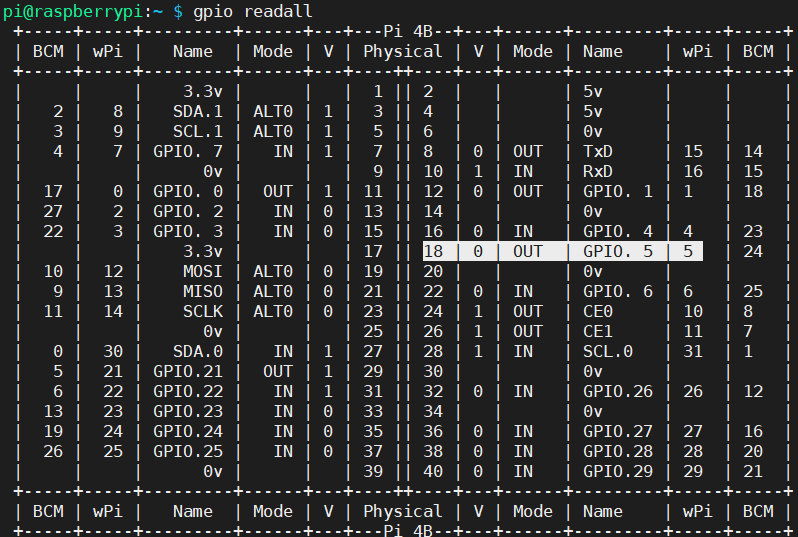
\includegraphics[width=\linewidth]{lernportfolio_assets/GPIO_Pins}
              \caption{Pin Mapping WiringPi Motorhat}
              \label{fig:boat1}
        \end{figure}
        Der Ultraschallsensor HC-SR04 hat einen Vcc, einen Gnd, einen Trigger und einen Echo Anschluss.
        Der Ultraschallsensor benötigt eine Versorungsspannung von 5 Volt,
        welche vom Motorhead bereitgestellt wird.
        Der Trigger wird mit dem GPIO Pin 5 des Motorhead bzw. mit dem Pin 21 der wiringPi Bibliothek verbunden.
        %TODO @Pierre Ist das hier korrekt umschrieben Pierre?
        Das Echo Signal wird vom Motorhead mit einer Spannung von 5V
        zurückgegeben. Da der RaspberryPi jedoch nur eine Spannung von 3,3V
        verträgt, ist die Verwendung eines Vorwiderstand von 330$\Omega$ nötig.
        Zusätzlich wird ein Pull-Down Widerstand in Höhe von 470$\Omega$
        angeschlossen, welcher den Pin gegen Ground zieht, um so ein floating state zu verhindern.
        Der GND Anschluss des Ultraschallsensors wird direkt an den GND Pin vom Motorhat angeschlossen.

        \begin{figure}
            \centering
            \begin{minipage}{0.45\textwidth}
                \centering
                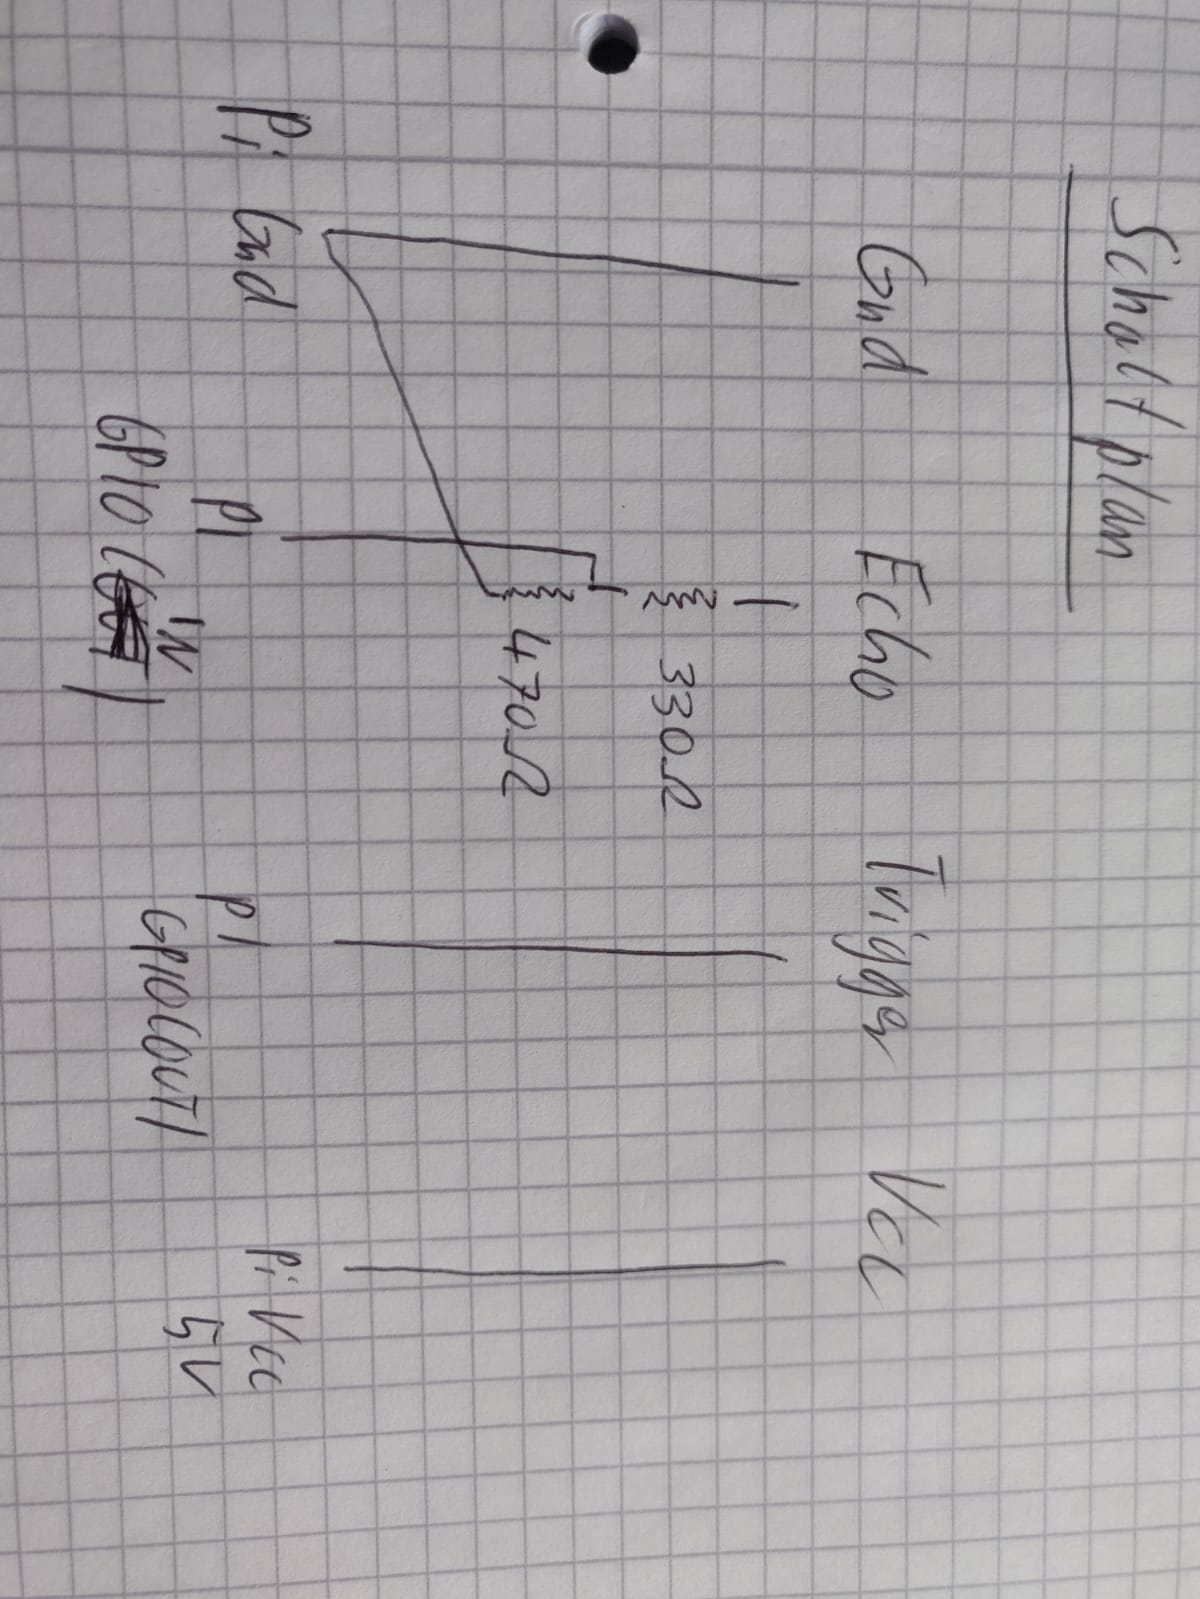
\includegraphics[width=0.9\textwidth]{lernportfolio_assets/Schaltplan_Ultraschallsensor1} % first figure itself
                \caption{Auf Papier}
            \end{minipage}
            \hfill
            \begin{minipage}{0.45\textwidth}
                \centering
                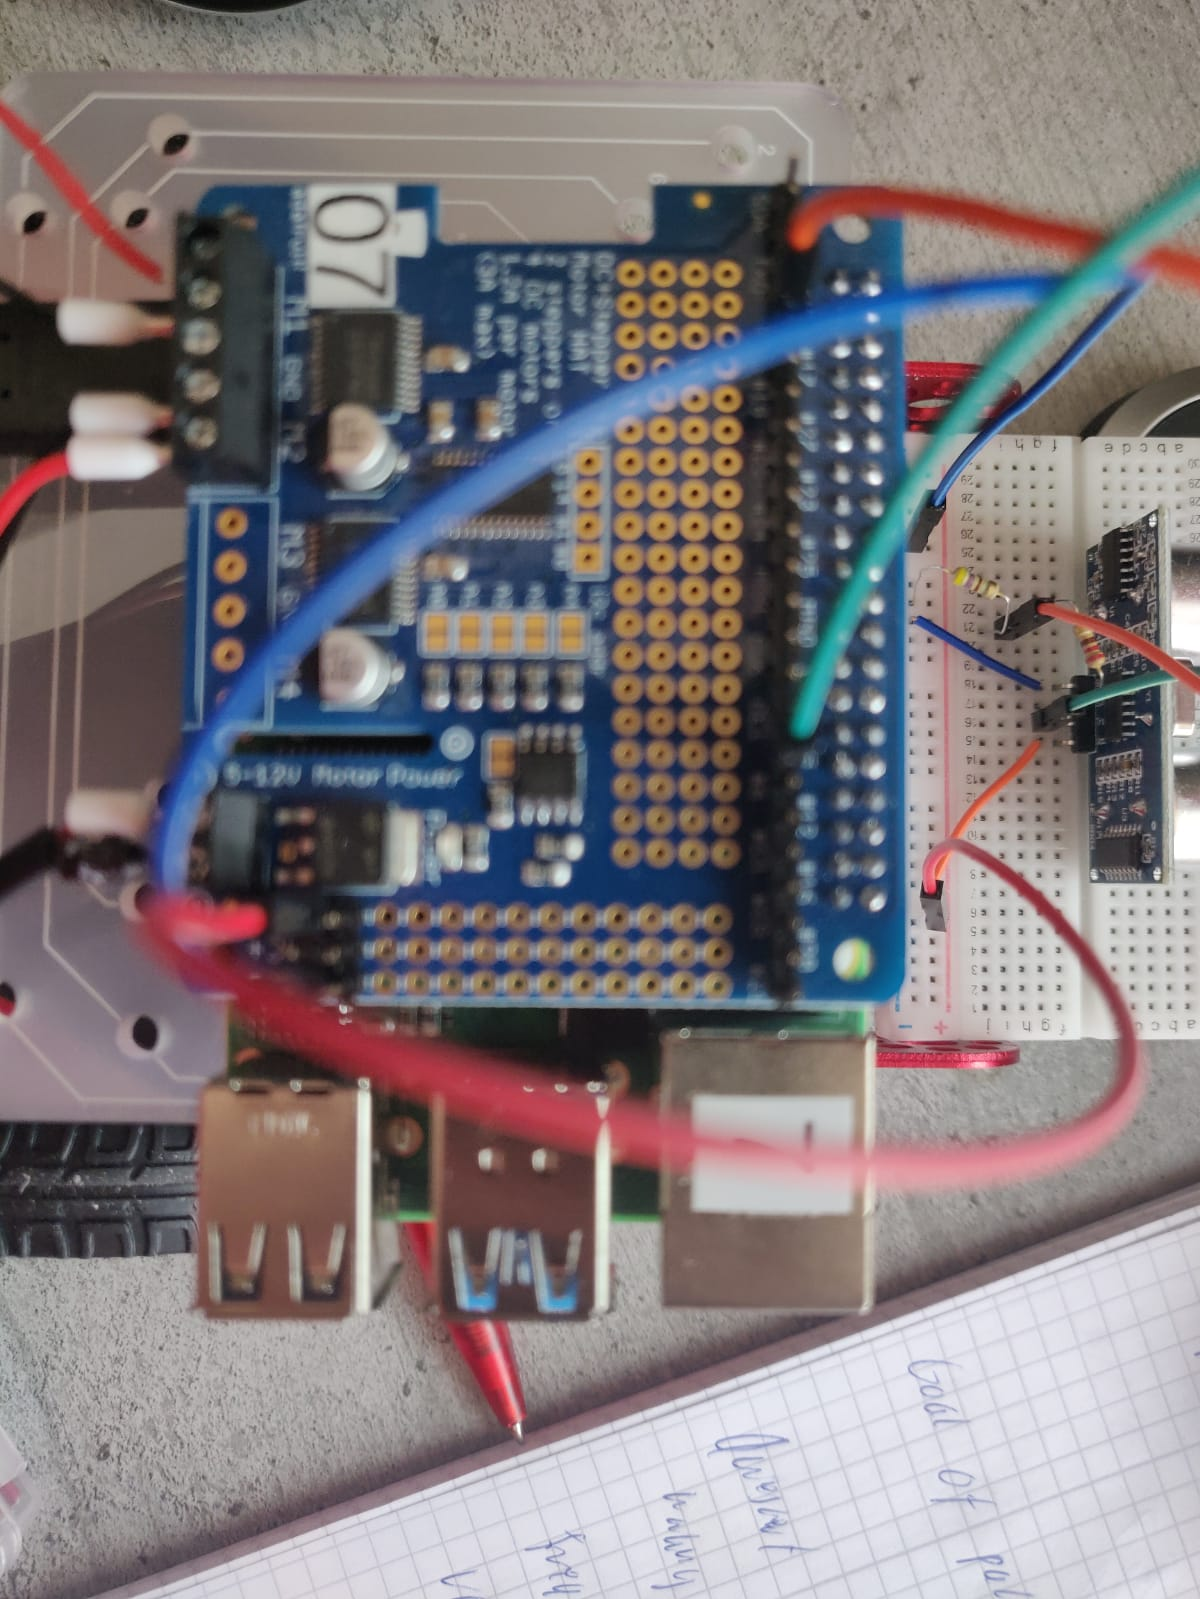
\includegraphics[width=0.9\textwidth]{lernportfolio_assets/Schaltplan_Ultraschallsensor2} % second figure itself
                \caption{Auf Papier}
            \end{minipage}
        \end{figure}
    \end{subsection}
    \begin{subsection}{Distanzberechnung}
        Die Distanz wird durch den Ultraschallsensor berechnet indem durch den Trigger ein Signal losschickt und die Zeit misst, die das Signal braucht um am Echo anzukommen. 
        Distanz (in \si\cm)= \( \frac{Signalzeit}{2} \) \si\second $ \cdot $ 34350 \( \frac{\si\cm}{\si\second} \)
    \end{subsection}

    \begin{subsection}{Bewertung der Zuverlässigkeit der Entfernungsmessung}
      Die Entfernungsmessung funktioniert für solide Objekte in einer Reichweite
      von 5 bis 100 cm zuverlässig. Für weniger solide Objekten, wie z.B. einer
      Pappierbox, hat der Sensor bei den Tests Probleme
      gehabt, die Entfernung richtig einzuschätzen. Oftmals kam es hierbei zu keinen Rückmeldungen an den Echo-Pin. Dieses
      Problem wurde durch ein Zeitlimit beim Warten auf den Echo-Pin gelöst und
      verwerfen der Messung falls das Zeitlimit überschritten wurde. Das
      Ermitteln der Entfernung beinhaltet mehrere Entfernungsmessungen. Somit
      ist das verwerfen einzelner Messungen durch ein überschreiten des
      Zeitlimits vertretbar. Aus den Messungen wird anschließend ein Mittelwert
      gebildet und zurückgegeben. Durch mehrmaliges Messen und bilden des
      Mittelwertes wird zugleich die relativ hohe Varianz zwischen einzelnen
      Messungen bei gleicher Distanz zum Objekt abgefangen.
    \end{subsection}
    \begin{subsection}{Bewertung der Genauigkeit}
      Die Entfernungsmessung funktioniert mit einer Standardabweichung von unter
      1,3 cm auf 100 cm genau.
      Die Rohdaten können im Anhang \ref{ultraschallsensorRohdaten} eingesehen werden.
      Im folgendem eine Zusammenfassung.
      %The table is generated by pandas
      \begin{table}[h!]
        \begin{tabular}{lrrrrrrr}
          % \toprule
          Abstand &       5cm &        10cm &        15cm &        20cm &        30cm &        50cm &       100cm \\
          % \midrule
          count &  100.000000 &  100.000000 &  100.000000 &  100.000000 &  100.000000 &  100.000000 &  100.000000 \\
          mean  &    4.668009 &    9.355380 &   13.951283 &   19.938128 &   30.418109 &   51.078758 &   99.553521 \\
          std   &    0.032030 &    0.305832 &    0.109583 &    0.060932 &    0.107799 &    0.482031 &    1.268841 \\
          min   &    4.650300 &    8.792790 &   13.804400 &   19.811500 &   30.079000 &   50.054500 &   91.353200 \\
          25\%   &    4.663265 &    9.122402 &   13.854150 &   19.880775 &   30.405600 &   50.820775 &   99.667750 \\
          50\%   &    4.664025 &    9.305280 &   13.912850 &   19.933800 &   30.450700 &   50.999200 &   99.878350 \\
          75\%   &    4.665242 &    9.658680 &   14.020900 &   19.983375 &   30.478350 &   51.518525 &   99.959425 \\
          max   &    4.979740 &    9.821430 &   14.231100 &   20.131400 &   30.566800 &   51.951700 &  100.912000 \\
          % \bottomrule
        \end{tabular}
        \caption{Zusammenfassung der Rohdaten. Alle Werte in cm.}
    \end{table}
    Aus der Tabelle geht hervor, dass der Abstand zu nahen
    Objekten (Abstand <= 20 cm) tendenziell unterschätzt wird, zu entfernteren
    Objekten hingegen geringfügig überschätzt. Eine Ausnahme bildet hier die
    Messreihe für den Abstand von 100 cm.
    
    Um den Mittelwert gibt es für alle Werte eine Standardabweichung von weniger
    als 1,3 cm. Die Messung sind daher präzise. Erwähnenswert ist, dass die
    Standardabweichung bei kleineren Distanzen sehr viel geringer ist als bei größeren.

    \begin{figure}[h!]
      \centering
      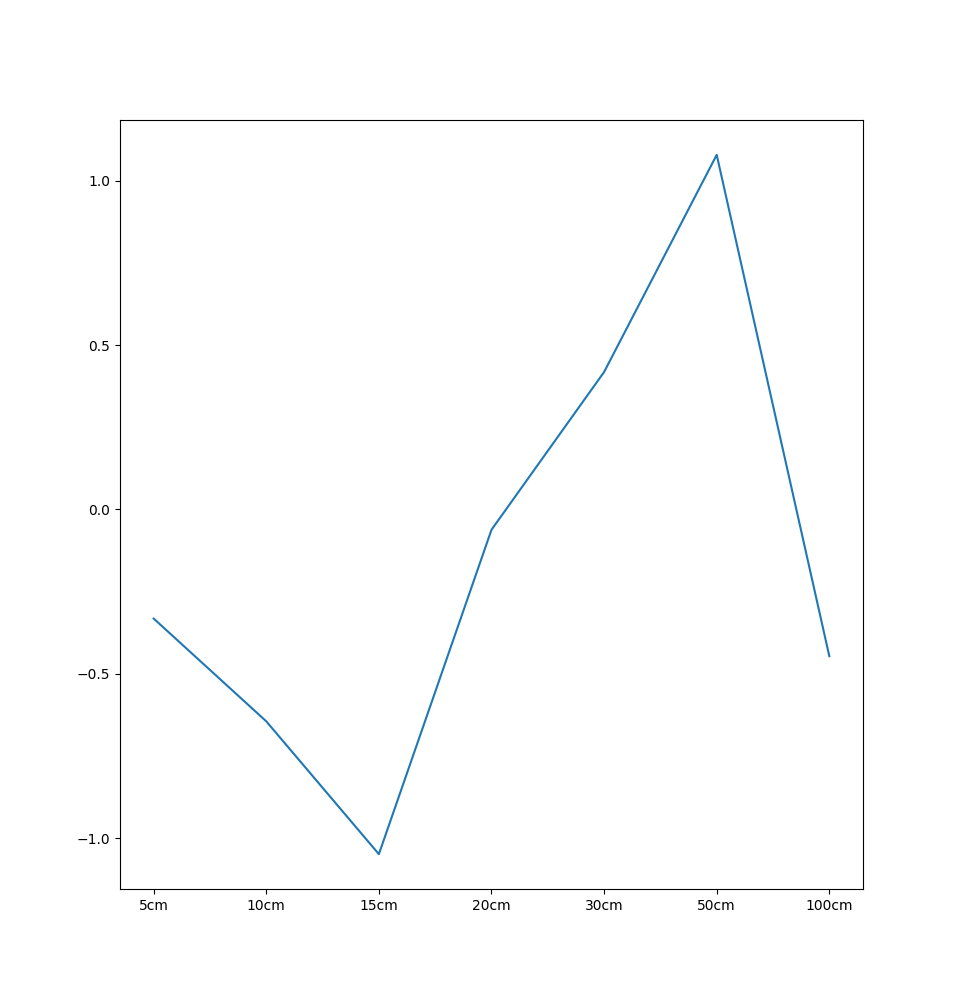
\includegraphics[width=0.5\textwidth]{test_data_ultrasonic/meanDiff.png}
      \caption{Differenz des Mittelwertes zur tatsächlichen Distanz}
    \end{figure}

  \end{subsection}

\end{section}

\begin{section}{Anhang}
  \begin{subsection}{Rohdaten Ultraschallsensor} \label{ultraschallsensorRohdaten}
    \input{test_data_ultrasonic/rohdaten.tex}
  \end{subsection}
\end{section}

\end{document}

 